\documentclass[]{standalone}
\usepackage[T1]{fontenc}
\usepackage{tikz}
\usepackage{amsmath, amsfonts}
\usetikzlibrary{arrows, shapes.geometric, calc, positioning, decorations.pathmorphing}

\makeatletter
\def\input@path{{./includes/}{./includes/ut/diags/}}
\makeatother

\tikzstyle{chainName} = [rectangle, rounded corners, minimum width=3cm, minimum height=1cm, text centered, draw=black]
\tikzstyle{block} = [rectangle, rounded corners, minimum width=1cm, minimum height=1cm, draw=black]
\tikzstyle{dots} = [inner sep=0pt, text height=10pt]
\tikzstyle{arrowParent} = [thick, ->, -to, shorten >= 2pt, shorten <= 2pt]
\tikzstyle{arrowRefl} = [dashed, ->, -to, shorten >= 2pt, shorten <= 2pt]
\tikzstyle{braceLL} = [decorate, decoration={brace,amplitude=6pt,mirror,raise=2pt}]
\tikzstyle{braceLR} = [decorate, decoration={brace,amplitude=6pt,raise=-8pt}]
\tikzstyle{ethBraceL} = [braceLL, sloped, rotate=180]
\tikzstyle{braceRR} = [decorate, decoration={brace,amplitude=6pt,raise=2pt}]
\tikzstyle{braceRL} = [decorate, decoration={brace,amplitude=6pt,raise=-8pt,mirror}]
\tikzstyle{ethBraceR} = [braceRR, sloped]


\begin{document}

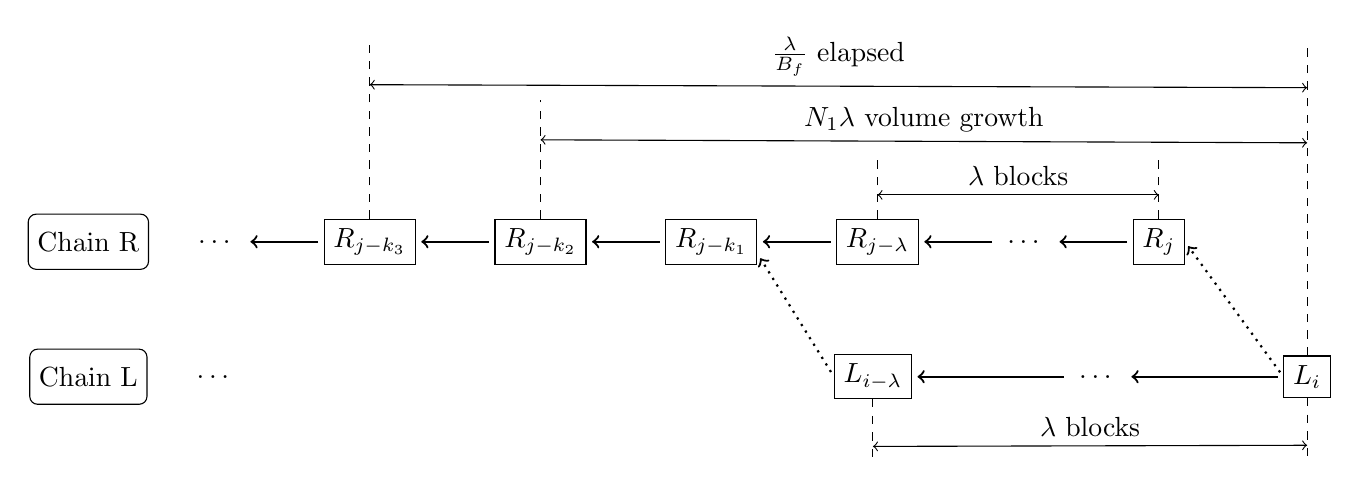
\begin{tikzpicture}[
roundednode/.style={rectangle,rounded corners=.1cm, draw=black!100, fill=white!5, thin, minimum size=7mm},
squarednode/.style={rectangle, draw=black!100, fill=white!5, thin, minimum size=2mm},
dotsnode/.style={draw=black!0, fill=white!5, minimum size=2mm},
]

%\draw[help lines] (-1,-5) grid (12,5);

%Nodes
\node[roundednode]      (chainr)                              {Chain R};
\node[dotsnode]      (chainrpast) [right=of chainr, xshift=-0.5cm]   {$\dots$};
\node[squarednode]      (remote4)  [right=of chainrpast]      {$R_{j-k_3}$};
\node[squarednode]      (remote3)  [right=of remote4]         {$R_{j-k_2}$};
\node[squarednode]      (remote2)  [right=of remote3]         {$R_{j-k_1}$};
\node[squarednode]      (remote1)  [right=of remote2]         {$R_{j - \lambda}$};
\node[dotsnode]      (remotex)  [right=of remote1]         {$\dots$};
\node[squarednode]      (remote0)  [right=of remotex]         {$R_j$};

\node[roundednode]      (chainl)   [below=of chainr]         {Chain L};
\node[dotsnode]      (chainlpast) [right=of chainl, xshift=-0.5cm]   {$\dots$};
\node[squarednode]      (local1)   [right=of chainlpast, xshift=6.5cm]         {$L_{i - \lambda}$};
\node[dotsnode]      (localx)   [right=of local1, xshift=1cm]          {$\dots$};
\node[squarednode]      (local0)   [right=of localx, xshift=1cm]          {$L_i$};

%Parent refs
\draw[arrowParent] (remote0.west) -- (remotex.east);
\draw[arrowParent] (remotex.west) -- (remote1.east);
\draw[arrowParent] (remote1.west) -- (remote2.east);
\draw[arrowParent] (remote2.west) -- (remote3.east);
\draw[arrowParent] (remote3.west) -- (remote4.east);
\draw[arrowParent] (remote4.west) -- (chainrpast.east);

\draw[arrowParent] (local0.west) -- (localx.east);
\draw[arrowParent] (localx.west) -- (local1.east);

\draw[dotted, black, arrowParent] (local0.west) -- (remote0.east);
\draw[dotted, black, arrowParent] (local1.west) -- ([yshift=-0.15cm]remote2.east);

%Dashed references
\draw[dashed] (remote4.north) -- +(0, 2.2);
\draw[dashed] (remote3.north) -- +(0, 1.5);
\draw[dashed] (remote1.north) -- +(0, 0.8);
\draw[dashed] (remote0.north) -- +(0, 0.8);

\draw[dashed] (local1.south) -- +(0,-0.8);
\draw[dashed] (local0.south) -- +(0,-0.8);
\draw[dashed] (local0.north) -- +(0,3.9);

%Condition arrows
\draw[black, arrows={<->}] ([yshift=-0.6cm]local0.south) -- ([yshift=-0.6cm]local1.south)
    node[midway, above] {$\lambda$ blocks};
\draw[black, arrows={<->}] ([yshift=0.3cm]remote0.north) -- ([yshift=0.3cm]remote1.north)
    node[midway, above] {$\lambda$ blocks};
\draw[black, arrows={<->}] ([yshift=2.7cm]local0.north) -- ([yshift=1.0cm]remote3.north)
    node[midway, above] {$N_1 \lambda$ volume growth};
\draw[black, arrows={<->}] ([yshift=3.4cm]local0.north) -- ([yshift=1.7cm]remote4.north)
    node[midway, above] {$\frac{\lambda}{B_f}$ elapsed};

\end{tikzpicture}

\end{document}
